\chapter{How to Achieve the Highest Processing Power in a Software Application}\label{chap:chap3}

\section*{}

In this chapter is explained the problem that describes this thesis' theme, what is the solution that will be proposed, the perspective and concepts behind the proposed solution and the methodology that will be used to achieve the proposed solution and how to validate this proposed solution. 

\section{Problem}

According to the state of the art presented in the previous chapter, giving a software application, how to make it as efficiently as it is possible, in terms of performance and energy cost, without jeopardizing its results and outcome in a heterogeneous systems? 


\section{Solution's Perspective}

In order to achieve such performance in the conditions mentioned in the problem's section, I purpose an autotuner or a concept proof that will enhance the application. For that, this autotuner will receive the program's original source code and though parallel optimization a new code will emerge. This code's modification will increase applications performance without jeopardizing the application's outcome.

\subsection{Solution's Approach}

To create this autotuner, the first step is to identify what parameters exist to tune and what impact they have in the application. For this matter, with the help of Kremlin and manual expert parallelization applications will increase its performance and parameters will be found. As Kremlin detect possible parallelized code and, additionally, measures the applications speedup with such modifications, and with manual expert parallelization, there will be a confront with these results and find what is better between these two scenarios. With this confrontation, and with different use cases, the tunning parameters will be found and the autotuner will be made.

\subsection{Solution's Methodology}
\begin{figure}[t]
  \begin{center}
    \leavevmode
    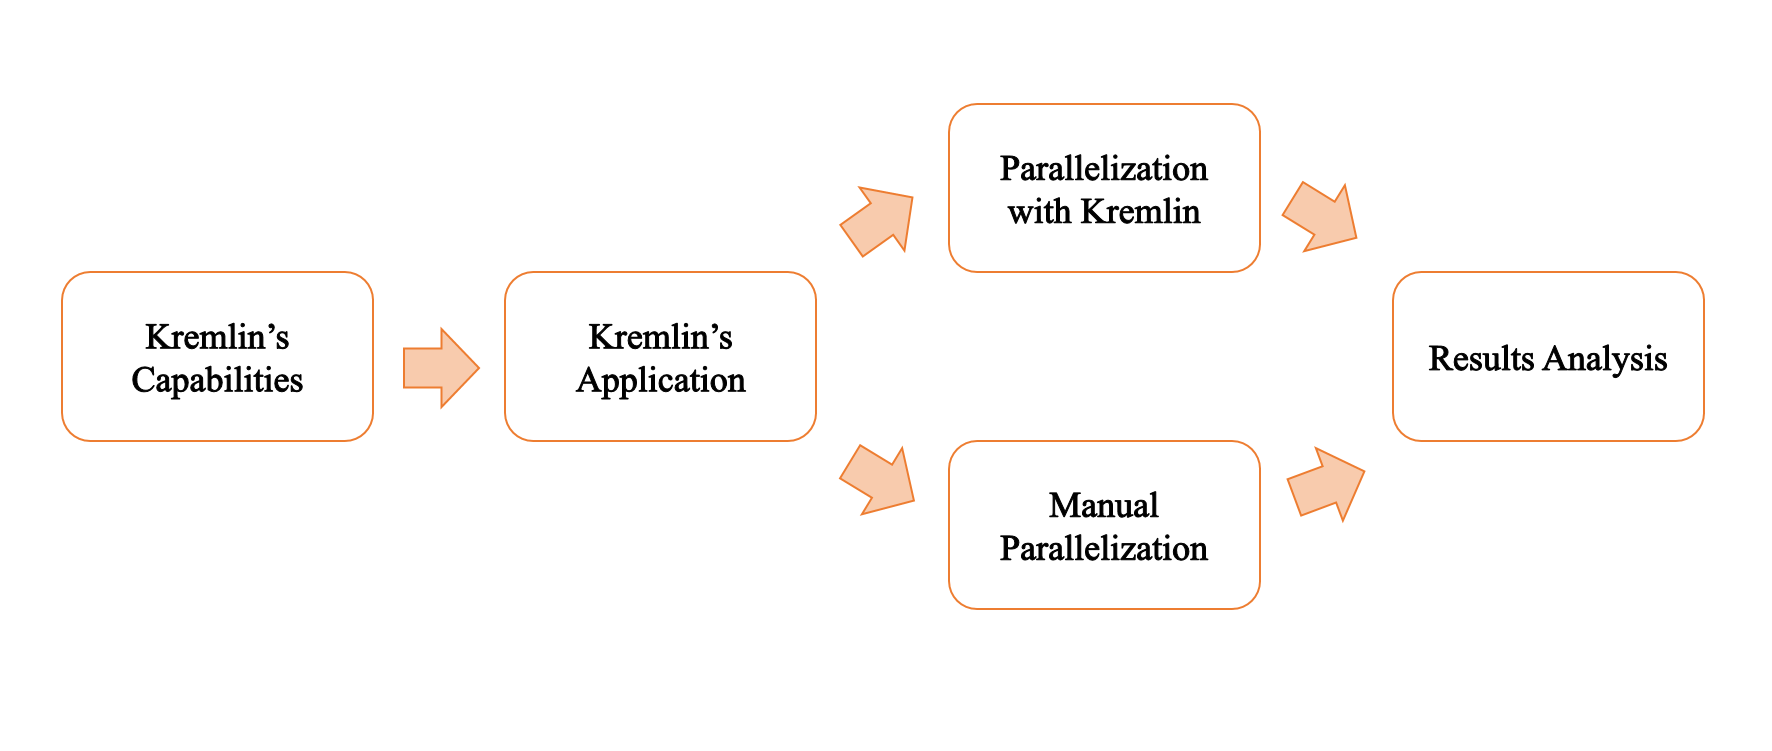
\includegraphics[width=1\textwidth]{methodology}
    \caption{Methodology that will be followed}
    \label{fig:method}
  \end{center}
\end{figure}

In the  figure ~\ref{fig:method} is outlined the steps that will be followed to create the autotuner. This methodology has six states. Firstly and using simple applications, an evaluation will be made for Kremlin to understand how to use this software tool and evaluate the results that Kremlin can achieve, for instance, if it has similar results comparing with a expert parallelizing manually the same code. Then Kremlin will be applied to specific applications. After this state, I will compare results with different Kremlin set ups and it is possible to return to the previous state to apply Kremlin but in a different configuration set up.

Simultaneously and for the same application, I will manually parallelized code in order to evaluate the results and compare with the Kremlin results. As these states (the experiences with Kremlin and the manual code parallelization) requires several attempts there will be transitions between manual and Kremlin states. 

The creations of the autotuner or concept proof happens when the tunning parameters are found after several attempts in the previous states. To make sure that the autotuner is being built correctly, evaluations will be made in order to verify the autotuner performance, so that the autotuner is correctly being made.

To sum up, this methodology as three main stages: learn and evaluate  Kremlin's uses and results; finding the tunning parameter thorough several attempts using Kremlin's outputs and manually parallelize the application's code, and compare and analyze the results in every attempt; and, in the end, the constructions of the autotuner.


\subsection{Solution's Validation}

To validate the whole methodology process, not only the autotuner itself but to compare the results between Kremlin outcomes and the code manually being parallelized, for evaluation metrics will be used: system energy consumptions when running the application; applications execution time; number of memory accesses and cache misses on the application; and the processing power measured by the number of instructions per secs. These evaluation metrics will be compared in three different cases: the original sequential code; manually paralleled code; and "automatic" paralleled code. In this last case it can be with Kremlin or with autotuner, depending in which of the methodology's state I am currently in.

To measure the above mentioned evaluation metrics, some libraries will be used: to measure energy consumptions RAPL will be used~\cite{Marcus}; to measure application  execution time OpemMP will be used ~\cite{Nc1998}; to measure number of memory accesses, cache misses and processing power PAPI ~\cite{Marcus} will be used.

Finally, two use cases will be used to validate this solution: a biopharmaceutical HPC application for accelerating drug discovery; and a self-adaptive navigation system to be used in smart cities. These use cases will be the applications that, the autotuner will try to achieve the highest processing power without jeopardizing the applications' outcome and having a low energy consumption.
